\documentclass[a4paper,10pt,oneside]{article}
\usepackage{graphicx}
\usepackage{color}
\usepackage{url}
\usepackage{subfigure}
\usepackage[utf8]{inputenc}
\usepackage[T1]{fontenc}
\usepackage{tgpagella}
%\usepackage[scale=0.9]{tgcursor}
%\usepackage[scale=0.9]{tgheros}
\usepackage{xstring}

\newcommand{\myscale}{0.74}
\newcommand{\vect}[1]{\boldsymbol{#1}}
\newcommand{\code}[1]{\texttt{\StrSubstitute{#1}{.}{.\.}}}
\def\.{\discretionary{}{}{}}
\newcommand{\jmodule}[1]{\emph{#1}}

\setlength{\hoffset}{-1in} %left margin will be 0, as hoffset is by default 1inch
\setlength{\voffset}{-1in} %analogous voffset
\setlength{\oddsidemargin}{1.5cm}
\setlength{\evensidemargin}{1.5cm}
\setlength{\topmargin}{1.5cm}
\setlength{\textheight}{24cm}
\setlength{\textwidth}{18cm}

\def\mftitle{jInfer XSDImporter Module Description}
\def\mfauthor{Michal Klempa, Mário Mikula, Robert Smetana, Michal Švirec, Matej Vitásek}
\def\mfadvisor{RNDr. Irena Mlýnková, Ph.D., Martin Nečaský, Ph.D.}
\def\mfplacedate{Praha, 2011}
\title{\bf\mftitle}
\author{\mfauthor \\ Advisors: \mfadvisor}
\date{\mfplacedate}

\ifx\pdfoutput\undefined\relax\else\pdfinfo{ /Title (\mftitle) /Author (\mfauthor) /Creator (PDFLaTeX) } \fi

\begin{document}
\maketitle
\noindent Target audience: developers willing to extend jInfer, specifically those creating or extending a parser.

\noindent \begin{tabular}{|l|l|} \hline
Responsible developer & Robert Smetana \\ \hline
Required tokens       & none \\ \hline
Provided tokens       & none \\ \hline
Module dependencies   & listed for each module separately \\ \hline
Public packages       & listed for each module separately \\ \hline
\end{tabular}

\section{Introduction}
This document focuses on the description of modules involved in the process of importing of XML Schema Definition (XSD) documents, or Schema documents. 
These modules are responsible for creating the IG rules from input files, therefore they belong in the inference modules category. 
As a whole, they are a specialized extension of \code{BasicIGG} module.

None of the modules provide nor require any tokens. Complete dependency tree is described in \cite[section 4]{archdoc} and depicted in figure 9 of that document.

\subsection{Naming convention}
Note that there are several types of entities called `element' in the context of the described modules.
To avoid ambiguity, in this document we shall use notation \code{DOM.Element} 
for instances of \code{org.w3c.dom.Element} and notation \code{Element} 
for instances of\code{cz.cuni.mff.ksi.jinfer.base.objects.nodes.Element}.

To add to this complication, XSD Schemas are XML documents which consist of elements and attributes.
We shall refer to these XML elements as \emph{tags} and XML attributes as \emph{tag attributes}.
Moreover, all tags and tag attributes that are known to our parsers are specified in
section \ref{sect:utils}.

For example, the \emph{attribute} tag can have a tag attribute \emph{use}.
While former will match \code{XSDTag.ATTRIBUTE}, the latter will match \code{XSDAttribute.USE}.
Lastly, tag attributes should not be confused with instances of \code{Attribute}, which is a class for storing information about the tag attributes inside jInfer. Every \code{Element} has a list of \code{Attribute}s, as can be seen from figure 4 in \cite[section 2.3]{archdoc}.

\subsection{Namespaces}
XSD Schemas allow using different namespace prefixes for tag names. Our parser implementations do not recognize namespaces; all prefixes from tag names are trimmed. For example, there is no difference between \code{xs:choice} and \code{xsd:choice} tags, both will match the \code{XSDTag.CHOICE} constant.

\subsection{Rule-trees} \label{sect:ruletree}

Rule-trees are tree data structures, where vertices are instances of \code{Element} class and edges are the relations between them stored in \code{Regexp} instances within vertices. Every vertex is a rule by itself, so in order to obtain IG rules, one must extract all Elements from a rule-tree. Rule-trees are created by \code{DOMHandler}, described in subsection \ref{sect:domhandler}. The extraction is done by \code{DOMParser}, described in subsection \ref{sect:domparser}. Or alternatively, when parsing with SAX is selected, \code{SAXHandler} handles both processes. 

Life cycle of rule-trees is apparent from section \ref{sect:dataflow}.

\section{Structure}
There are three modules that provide support for importing Schema files bundled with jInfer. 
\begin{itemize}
	\item \code{XSDImporter} - Main module providing support for actual parsing modules, as well as common configuration options for the parsers.
	\item \code{XSDImportDOM} - Dependent module implementing DOM parser method.
	\item \code{XSDImportSAX} - Dependent module implementing SAX parser method. 
\end{itemize}
All three modules depend on the \code{Base} module, as they all use the common data structures of jInfer. 
\code{XSDImporter} module also depends on \code{BasicIGG} module.
DOM and SAX parser modules are independent of each other; 
however, they rely on classes from \code{XSDImporter}. 
They provide similar functionality, but use different paradigms.

\subsection{XSD Importer module}

\noindent \begin{tabular}{|l|l|} \hline
Module dependencies:   & Base \\ 
                       & BasicIGG \\ \hline
Public packages:       & cz.cuni.mff.ksi.jinfer.xsdimporter.interfaces \\
                       & cz.cuni.mff.ksi.jinfer.xsdimporter.utils \\ \hline
\end{tabular}
\\

\noindent This module has several key roles in the process of importing XSD documents.\\

Firstly, it is an extension of the \code{BasicIGG} module, registering a service provider
of a \code{Processor} class, to handle files with \emph{xsd} extension (see \cite[section 3]{basiciggdoc}). 
It defines a common interface providing the developers with easy integration of their custom parsers to the rest of the inference process.
It also provides a common configuration in the form of a properties panel in project properties for all depending modules.
And finally, this module holds common utility classes related to the task of processing data characteristic to the Schema documents. \\
Functionality is divided between separate packages, in the same order as above:

\begin{itemize}
	\item \code{cz.cuni.mff.ksi.jinfer.xsdimporter}
	\item \code{cz.cuni.mff.ksi.jinfer.xsdimporter.interfaces}
	\item \code{cz.cuni.mff.ksi.jinfer.xsdimporter.properties}
	\item \code{cz.cuni.mff.ksi.jinfer.xsdimporter.utils}
\end{itemize}

Since some of the packages contain only one important class, we structure the documentation in logical blocks based on significance, not package structure.

\subsubsection{XSD Processor}

Similar to the \code{Processor} implementations in the \code{BasicIGG} module, this is the core class of \code{XSDImporter} logic.
\code{XSD\.Pro\.cessor} registers itself into \emph{schema} input folder, \emph{xsd} file extension and declares it cannot handle other file extensions.\\
Class depends on NBP lookups (see \cite[section 4.1]{archdoc}) to find available parsers, and uses the selected parser to perform the import operation on defined files.
Initial grammar generated by this processor is considered \emph{complex} and should be followed by expansion if necessary (see \cite[section 4]{basiciggdoc}).

\subsubsection{XSD Parser interface}

Key interface which needs to be implemented by any parser handling the import of Schema documents. Lookups of available parsing methods work by searching for service providers based on this interface. In order to support the lookup functionality, this interface extends \code{NamedModule}. It declares method \code{parse()} which takes an \code{InputStream} that contains the input document and returns a complete list of rules from that document. In other words, this method does all the necessary work. Method has the following signature:

\begin{verbatim}
List<Element> parse(InputStream stream) throws XSDException;
\end{verbatim}

Diagram showing the inheritance of this interface, as well as both parsers bundled with jInfer, which implement it is in figure \ref{parser_interface}.

\begin{figure}[ht]
\centering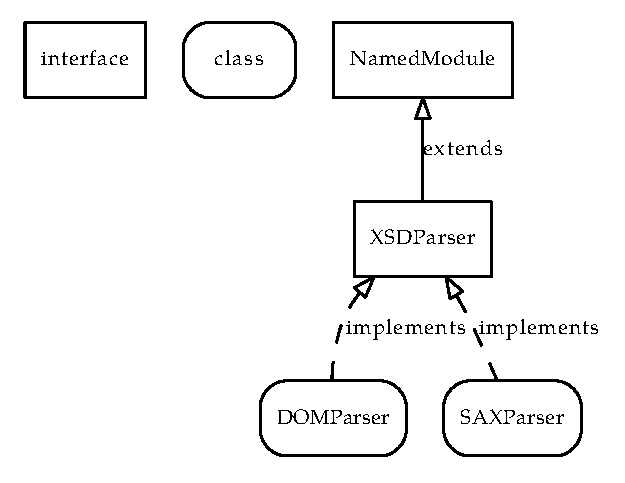
\includegraphics[scale=\myscale]{parser_intf}
\caption{Inheritance of XSDParser interface.} \label{parser_interface}
\end{figure}

\subsubsection{Properties}

Settings provided by the package \code{cz.cuni.mff.ksi.jinfer.xsdimporter.properties} are project-wide.
They are meant to be common for all parsers handling the import of Schema documents. Access to these settings is provided by utility class \code{XSDImportSettings} described in section \ref{sect:utils}. For description of each of the settings, please see section \ref{sect:settings}.

\subsubsection{Utils} \label{sect:utils}

Package \code{cz.cuni.mff.ksi.jinfer.xsdimporter.utils} contains classes available to all parsing methods.

\paragraph{Built-in data types}

A special class is designed to contain all built-in data types supported by XSD language. Both built-in primitive types and built-in derived types are recognized. For a complete list, please see our JavaDoc documentation for \code{XSDBuiltInDataTypes} class. These types are contained using instances of \code{SimpleData} class, as described in \cite[section 2.2]{archdoc}.

\paragraph{XSD Import Settings} 

Simple utility class that provides convenient access methods to all the settings, hiding unnecesary implementation details. It holds the following methods.

\begin{itemize}
	\item \code{getParser()} returns selected instance of \code{XSDParser}.
	\item \code{logLevel()} returns current log priority, messages with lower priority are not displayed.
	\item \code{isVerbose()} returns \code{true} or \code{false}, depending on state of the checkbox.
	\item \code{stopOnError()} returns \code{true} or \code{false}, depending on state of the checkbox.
\end{itemize}

\paragraph{XSD Occurences}

Helper class for creating intervals from string representation of occurrences found in \code{minOccurs} and \code{maxOccurs} attributes of schema tags. Default values for both attributes are 1. Methods can create all types of intervals. If optional flag \code{minHasPriority} is set, method \code{createInterval} will prefer the value of lower bound, if parsing of upper bound fails, which can result in an interval with equal values of lower and upper limit (\code{min, min}).

\paragraph{XSD Attribude}

Enumeration of tag attributes currently recognized by our parsers. They are the following.
\begin{itemize}
	\item \code{name}
	\item \code{ref}
	\item \code{type}
	\item \code{use}
	\item \code{minOccurs}
	\item \code{maxOccurs}
\end{itemize}
List should be extended according to the parser, to reflect its functionality.

\paragraph{XSD Tag}

Enumeration of tags currently known by our parsers. They are the following.
\begin{itemize}
	\item \code{schema}
	\item \code{element}
	\item \code{complexType}
	\item \code{sequence}
	\item \code{choice}
	\item \code{all}
	\item \code{attribute}
	\item \code{redefine} - this tag is not yet supported, but allows parsing of a certain types of documents
\end{itemize}
This list should also be updated in case the parser functionality is extended.

\paragraph{XSD Utility}

This is basically only a library of short, useful and frequently used functions for parsing, please refer to the JavaDoc.

\paragraph{XSD Exception}

\code{XSDException} is a simple class extending \code{RuntimeException} to announce errors during import operation. It is catched by \code{XSDProcessor} which checks if \emph{Stop on error} setting is enabled and stops the inference.

\subsection{XSD Import DOM module}

\noindent \begin{tabular}{|l|l|} \hline
Module dependencies:   & Base \\ 
                       & XSDImporter \\ \hline
Public packages:       & none \\ \hline
\end{tabular}
\\

\noindent This module implements the import functionality using API from Xerces DOM parser. Its structure is very simple, all classes are grouped in one main package, relying on utility classes from \code{XSDImporter} module mentioned before.

\subsubsection{DOM Parser} \label{sect:domparser}
Class implementing \code{XSDParser} interface. It is responsible for creation of DOM tree, extraction of contained rule-trees and aggregation of rules from them. First task is delegated to the underlying Xerces DOM parser API. Conversion between DOM tree and the rule-trees is then passed to \code{DOMHandler}. 

\begin{verbatim}
parser = new com.sun.org.apache.xerces.internal.parsers.DOMParser();
parser.parse(new InputSource(stream));
Document doc = parser.getDocument();
DOMHandler handler = new DOMHandler();
List<Element> ruleTrees = handler.createRuleTrees(doc.getDocumentElement());
\end{verbatim}

\subsubsection{DOM Handler} \label{sect:domhandler}
When DOM parsing method is selected, most of the logic is implemented in \code{DOMHandler} class.
This class is responsible for creating so called rule-trees from an existing Document Object Model.

Its only public method iterates through children of the root node, given as parameter, in two passes. This root node should always contain \code{schema} tag, according to XSD specification. Firstly, it registers \code{complexType} and \code{element} tags, as these can be referenced from within the tree. And then launches the algorithm for creating rule-trees for relevant nodes. It can be summarized as follows:

\begin{verbatim}
public List<Element> createRuleTrees(org.w3c.dom.Element root) {
  for each (root.getChildNodes() as tag) {
    if (tag = XSDTag.ELEMENT)     addToReferenced(tag);
    if (tag = XSDTag.COMPLEXTYPE) addNamedCType(tag);
  }
  for each (root.getChildNodes() as tag) {
    subtree = buildRuleSubtree(tag);
    ruleTrees.add(subtree);
  }
  return ruleTrees;
}
\end{verbatim}

The most important method is \code{buildRuleSubtree()}. It is divided into four logical parts.
\begin{enumerate}
	\item Creates an \code{Element} instance with appropriate parameters (occurences, metadata, etc.).
	\item Inspects the given tag and sets parameters for subnodes \code{Regexp}.
	\item Recursively creates rule-subtrees for its children.
	\item Finalizes the instance by checking for extra conditions.
\end{enumerate}

Signature of the method is:
\begin{verbatim}
private Pair<Element, RegexpInterval> buildRuleSubtree(
          org.w3c.dom.Element currentNode,
          List<String> context,
          List<org.w3c.dom.Element> visited) throws XSDException
\end{verbatim}

Method takes current node, which will be returned as root \code{Element} node (first value of the returned pair) of this subtree, and creates an entire rule-tree below it by recursively calling itself, as mentioned in step 3. Context parameter holds the list of names of nodes that create unique path from actual root of the schema document to the current node. Visited parameter lists references to instances of \code{Element} that were visited on this path. When handling \emph{attribute} tags, context needs to be passed along, but list of visited nodes does not.

\subsubsection{DOM Helper}
Helper class for \code{DOMHandler}, containing ulility functions specific for DOM parsing method.
Two most notable of them are \code{createSentinel()} and \code{finalizeElement()}.

\begin{description}
	\item[CreateSentinel()] Creates an instance of \code{Element} class, which is always a leaf in the rule-tree. This is useful when there are cyclic definitions in an input Schema document, or an \code{Element} with this name was defined previously and it is unnecessary to build a rule subtree for it again (it is a reference in this case). More information about sentinels can be found in \cite[section 3.2]{archdoc}, or \cite[section 4]{twostepdoc}.
	\item[FinalizeElement()] Checks if \code{Element} is properly defined. Redefine it to \code{LAMBDA} when it was empty, or to token if it only contained a simple data type. This method allows for built-in data types of tags to be retained for export.
\end{description} 

\subsection{XSD Import SAX module}

\noindent \begin{tabular}{|l|l|} \hline
Module dependencies:   & Base \\ 
                       & XSDImporter \\ \hline
Public packages:       & none \\ \hline
\end{tabular}
\\

\noindent This module implements the import functionality using API of a standard SAX parser. Its structure is divided in two packages. Package \code{cz.cuni.mff.ksi.jinfer.xsdimportsax} holds the main parsing logic, while package \code{cz.cuni.mff.ksi.jinfer.xsdimportsax.utils} contains two utility classes. Both \code{SAXAttributeData} and \code{SAX\.Do\.cu\.ment\.Ele\.ment} serve as wrappers for tag attributes and tags of the input Schema file during parsing, to ease the process of extracting data from them.

Classes \code{SAXParser} and \code{SAXHelper} are very similar to their counterparts in \code{XSDImportDOM} module, for information about their methods please refer to the JavaDoc. Implementation is also relying on utility classes from \code{XSDImporter} module mentioned before.

\subsubsection{SAX Handler}

Sax handler implements methods in response to the events generated by the underlying SAX parser API.
Similar to its counterpart, \code{DOMHandler}, this class holds most on the logic for importing a Schema.
It works by keeping current tree branch, which is being parsed, on a stack. Adding current node to the parent on top of the stack as current tag finishes.


\section{Data Flow}
Parsing of XSD begins when \code{IGGeneratorImpl} calls \code{XSDProcessor} with an input file.
The overall data flow while parsing a Schema document is simple, it can be summarized into following steps.
\begin{enumerate}
	\item \code{XSDProcessor} finds out the selected \code{XSDParser} from available service providers. This also indicates which module will be handling the actual parsing.
	\item \code{XSDProcessor} passes the input document to a selected module by calling \code{parse()} method on the selected \code{XSDParser}.
	\item Depending on the module, the corresponding API is used to extract IG rules from the input document.
	\item List of rules that were extracted from the document are returned to \code{XSDProcessor}.
	\item If no errors occured during this process, list of extracted rules is returned to \code{IGGeneratorImpl} for expansion. Otherwise, depending on the \emph{Stop on error} setting, the inference is stopped, or an empty list of rules for this input document is returned.
\end{enumerate}

\subsection{Data Flow using DOM parser}
When using the DOM parsing method, extraction of rules from a Schema document, mentioned in step 3 above, proceeds as follows.
\begin{enumerate}
	\item Document Object Model tree data structure is created from the input file by \emph{Xerces DOM parser}.
	\item Root node of the DOM tree is handed over to \code{DOMHandler} class.
	\item \code{DOMHandler} recursively passes the DOM tree by a depth-first algorithm and creates complete subtrees of rules (rule-trees) for each of the direct children of root node.
	\item Rule-trees are returned from \code{DOMHandler}.
	\item \code{DOMParser} traverses the returned rule-trees depth-first to create a list of final rules. Each of the rules now contains a full path, thanks to the way in which they were created.
\end{enumerate}

\subsection{Data Flow using SAX parser} \label{sect:dataflow}

Due to the nature of SAX parser paradigm, it is not possible to create the tree data structure in the top-to-bottom fashion, as with DOM parser. However, using stack data structures, analogous rule-trees are created from bottom to top, leading to a similar data flow. 

\begin{enumerate}
	\item A \code{SAXParserFactory} is created and our implementation of handler class \code{SAXHandler} is passed to it, along with \code{InputStream} containing an input document.
	\item Our handler then sequentially responds to events generated by the SAX parser, creating \code{Element} nodes when appropriate, and keeping them on a stack. This way, a relation can be created by adding an \code{Element} as a child to the \code{Element} on top of the stack.
	\item When parsing is finished, the rule-trees are kept in the data structures of \code{SAXHandler}.
	\item \code{SAXParser} calls \code{getRules()} method of \code{SAXHandler} to traverse the rule-trees to create the list of final rules in a similar manner as in DOM case. These rules also contain a full path.
\end{enumerate}


\section{Known issues and limitations} \label{sect:issues}

In this section we describe known problems that can occur while importing Schema documents. Supported structures are discussed only; tags and tag attributes that are not supported are not in scope of this section.

\subsection{SAX parser limitations}

Due to the inherent difficulty of SAX parsing method to cope with cross-referencing definitions, there is a known issue when schema defines \emph{complexType} tags in the following manner.

\begin{verbatim}
<xsd:complexType name="folderType">
  <xsd:sequence>
    <xsd:element name="file" type="fileType"/>
  </xsd:sequence>
</xsd:complexType>

<xsd:complexType name="fileType">
  <xsd:attribute name="ID" type="xsd:ID"/>
</xsd:complexType>

<xsd:element name="folder" type="folderType"/>
\end{verbatim}

In this example definition, the \code{folderType} type is dependent on \code{fileType} type, which has not been defined when a new Element, named \code{file}, is trying to resolve its type. This results in the parser assigning empty children to the \code{file} Element, adding the Element to a list of unresolved Elements and continuing with the parsing process. When parser reads the complete definition of \code{folderType} type, the type is only added to a list of known types, as there are no data structures for listing type cross-dependencies. 

When the complete definition of \code{fileType} is read, this type is also only added to a list of known types, no dependencies are retrospectively resolved.
The reason for it lies in one-pass approach of SAX parser. In future versions, we are planning to resolve this issue by creating dependency trees of \code{complexType} tag definitions. However, it will make the parsing algorithm more time and memory expensive.\\

Known fix is to place definitions of dependent types after the types they depend on have been defined, or simply using DOM parser, which is devoid of such complications by design. Using either will result in a desired output:

\begin{verbatim}
<xs:complexType name="Tfile">
  <xs:attribute name="ID" type="xs:ID"/>
</xs:complexType>

<xs:complexType name="Tfolder">
  <xs:sequence>
    <xs:element name="file" type="Tfile"/>
  </xs:sequence>
</xs:complexType>

<xs:element name="folder" type="Tfolder"/>
\end{verbatim}

\section{Settings} \label{sect:settings}

Common settings of modules can be found in project properties under \emph{XSD Import} category. They are project specific. Following list explains their purpose. 

\begin{description}
	\item[Parsing method] Setting selects whether SAX or DOM parser is used. 
This selection is based on the number of registered service providers for the \code{XSDParser} class,
so that both the jInfer bundled parsers as well as any custom parsers will be automatically displayed here.
DOM parser is set as the default parsing method. 
	\item[Log level] Setting determines the minimal priority for a message from the selected parser module to be logged. For example, if the module provides extensive debug information about elements being currently parsed, these messages can be filtered by setting the log level higher than \code{DEBUG}.
	\item[Stop on error] Checkbox determines if parsing halts the inference on the first error. If it is not set, then the file that caused the error is simply skipped and not imported. 
	\item[Print verbose info] Setting enables logging of some additional information, for example, complete list of imported rules, or extended warning messages.
\end{description}

\section{Extensibility} \label{sect:extensibility}

Module \code{XSDImporter} itself is an example of an extension of \code{BasicIGG}, for which it provides a specific funcionality. Other modules that handle different definition languages can be created in a similar fashion.

The modular design of the parser implementations is also an example of extensibility which can be achieved using the NetBeans platform. It allows developers to add, or remove, custom parsers just by creating a module with a new parser implementation; there is no need to change any code within \code{XSDImporter} module. Only exception is the re-definition of the default parser (currently DOM), which is not needed even if the module of default parser is not present.\\
Parsers with extended or custom functionality can be created using \code{XSDImportDOM} module as example (recomended).

\nocite{*}
\newpage
\bibliographystyle{alpha}
\bibliography{literature}

\end{document}
